\synctex=1
\documentclass[12pt]{article}
% Import geometry for smaller top
\usepackage{geometry}
% Required for inserting images
\usepackage{graphicx}
\graphicspath{{./images/}}
% Header and footer
\usepackage{fancyhdr}
% Language setting
\usepackage[utf8]{inputenc}
\usepackage[T2A]{fontenc}
\usepackage[russian]{babel}
% For better list
\usepackage{enumitem}
% For correct math operation
\usepackage{amsmath}
\usepackage{hyperref}
\usepackage{listings}

\geometry{a4paper,
 total={170mm,257mm},
 left=20mm,
 top=30mm,
 bottom=25mm
}

\fancypagestyle{first style}
{
\chead{\footnotesize{Санкт-Петербургский Национальный Исследовательский Университет ИТМО\\Факультет Технологического Менеджмента и Инноваций}}
\cfoot{\footnotesize{Санкт-Петербург 2025г.}}
\renewcommand{\headrulewidth}{0pt}
}

\begin{document}

\pagestyle{fancy}
\thispagestyle{first style}

\centering{
\includegraphics[scale=0.5]{LogoITMO}}

\vspace{25mm}

\centering{Вариант №14\\Лабораторная Работа №4\\По дисциплине\\Вычислительная математика}

\vspace{50mm}

\begin{flushright}
Выполнил студент группы P3218:\\Хромов Даниил Тимофеевич\\
\vspace{5mm}
Преподаватель:\\Бострикова Дарья Константиновна\\
\end{flushright}

\newpage

\pagestyle{empty}
\raggedright

\textit{Цель работы:} найти функцию, являющуюся наилучшим приближением заданной табличной функции по методу наименьших квадратов.\\

\section{Вычислительная реализация задачи}

\subsection*{\textit{Линейная аппроксимация}}
\vspace{5mm}
\[ y = \frac{25x}{x^4 + 14},\ x \in [0,4],\ h = 0,4;\ n = 11 \]
\vspace{5mm}
\centering
\begin{tabular}{ |c|c|c|c|c|c|c|c|c|c|c|c| }
  \hline
  i & 1 & 2 & 3 & 4 & 5 & 6 & 7 & 8 & 9 & 10 & 11\\
  \hline
  $x_i$ & 0 & 0,4 & 0,8 & 1,2 & 1,6 & 2,0 & 2,4 & 2,8 & 3,2 & 3,6 & 4,0 \\
  \hline
  $y_i$ & 0 & 0,684 & 1,332 & 1,792 & 1,868 & 1,6 & 1,221 & 0,89 & 0,646 & 0,475 & 0,356 \\
  \hline
\end{tabular}\\
\raggedright

Давайте теперь приступим к основной задаче аппроксимации, чтобы данную функцию $f(x)$ приближенно заменить (аппроксимировать) некоторой функцией $\phi(x)$, значения которой в заданной области мало отличались от опытных данных:
\[ \phi(x) = a + bx \]

Вычислим суммы: $SX = 22$, $SXX = 61,6$, $SY = 10,865$, $SXY = 20,302$\\

Теперь найдем коэффициенты $a$ и $b$, составив и решив следующую систему постановкой полученных значений:
\begin{equation}
  \begin{cases}
    11 \cdot a + 22 \cdot b = 10,865,\\
    22 \cdot a + 61,6 \cdot b = 20,302
  \end{cases}
\end{equation}

\begin{equation}
  \begin{cases}
    x = \frac{2173}{2200} - 2b,\\
    22 * \left( \frac{2173}{2200} - 2b \right) + 61,6b = 20,302
  \end{cases}
\end{equation}

Решая отдельно второе уравнение, где у нас одна зависимая переменная, получаем:
$$ 17,6y = -\frac{357}{250} $$
$$ y = -\frac{357}{4400} $$

Теперь подставим полученное значение в первое уравенение, где мы уже выразили $x$ и найдем его:
$$ x = \frac{2173}{2200} - 2 * \left( -\frac{357}{4400} \right) $$
$$ x = \frac{23}{20} $$

Тогда заключая получим:\\

\begin{equation}
  \begin{cases}
    x = \frac{23}{20},\\
    y = -\frac{357}{4400}
  \end{cases}
\end{equation}

Тогда наша приближенная функция будет иметь вид: $\phi(x) = -0,0811 * x + 1,15$.\\

\centering
\begin{tabular}{ |c|c|c|c|c|c|c|c|c|c|c|c| }
  \hline
  i & 1 & 2 & 3 & 4 & 5 & 6 & 7 & 8 & 9 & 10 & 11\\
  \hline
  $x_i$ & 0 & 0,4 & 0,8 & 1,2 & 1,6 & 2,0 & 2,4 & 2,8 & 3,2 & 3,6 & 4,0 \\
  \hline
  $y_i$ & 0 & 0,684 & 1,332 & 1,792 & 1,868 & 1,6 & 1,221 & 0,89 & 0,646 & 0,475 & 0,356 \\
  \hline
  $\phi(x_i)$ & 1,15 & 1,117 & 1,085 & 1,053 & 1,02 & 0,9878 & 0,955 & 0,923 & 0,89 & 0,858 & 0,826 \\
  \hline
  $(\phi(x_i) - y_i)^2$ & 1,322 & 0,188 & 0,061 & 0,546 & 0,719 & 0,375 & 0,07 & 0,001 & 0,0597 & 0,147 & 0,221 \\
  \hline
\end{tabular}\\
\raggedright
\vspace{5mm}
Тогда среднеквадратичное отклонение будет равно:
$$ \sigma = \sqrt{\frac{\sum_{i=1}^n (\phi(x_i) - y_i)^2}{n}} = \sqrt{\frac{3,7105}{10}} \approx 0,378 $$

\subsection*{\textit{Квадратичная аппроксимация}}
\[ y = \frac{25x}{x^4 + 14},\ x \in [0,4],\ h = 0,4;\ n = 11 \]

\centering
\begin{tabular}{ |c|c|c|c|c|c|c|c|c|c|c|c| }
  \hline
  i & 1 & 2 & 3 & 4 & 5 & 6 & 7 & 8 & 9 & 10 & 11\\
  \hline
  $x_i$ & 0 & 0,4 & 0,8 & 1,2 & 1,6 & 2,0 & 2,4 & 2,8 & 3,2 & 3,6 & 4,0 \\
  \hline
  $y_i$ & 0 & 0,684 & 1,332 & 1,792 & 1,868 & 1,6 & 1,221 & 0,89 & 0,646 & 0,475 & 0,356 \\
  \hline
\end{tabular}\\
\raggedright
\vspace{5mm}
Теперь нам нужно будет найти аппроксимирующую функцию вида:
\[ \phi(x) = a + bx + cx^2 \]

Снова вычислим суммы: $SX = 22$, $SXX = 61,6$, $SXXX = 193,6$, $SXXXX = 648,525$, $SY = 10,865$, $SXY = 20,302$, $SXXY = 47,198$\\

Теперь решим следующую систему для нахождения коэффициентов $a$, $b$ и $c$:

\begin{equation}
  \begin{cases}
    n * a * sx * b + sxxx * c = sy,\\
    sx * a + sxx * b + sxxx * c = sxy,\\
    sxx * a + sxxx * b + sxxxx * c = sxxy
  \end{cases}
\end{equation}

Подставим найденные раньше суммы в систему и продолжим вычисления:
\begin{equation}
  \begin{cases}
    11 * a + 22 * b + 61,6 * c = 10,865,\\
    22 * a + 61,6 * b + 193,6 * c = 20,302,\\
    61,6 * a + 193,6 * b + 648,525 * c = 47,198
  \end{cases}
\end{equation}

Решим систему с помощью метода Крамера:\\
\[ \Delta = 4252,424; \Delta_1 = 1203,834; \Delta_2 = 5799,063; \Delta_3 = -1536,022 \]

Теперь найдем коэффициенты нашей системы:
\begin{equation}
  \begin{cases}
    a = \frac{\Delta_1}{\Delta} = \frac{1203,834}{4252,424} \approx 0,283,\\
    b = \frac{\Delta_2}{\Delta} = \frac{5799,063}{4252,424} \approx 1,364,\\
    c = \frac{\Delta_3}{\Delta} = \frac{-1536,022}{4252,424} \approx -0,361
  \end{cases}
\end{equation}

Т.о. наша функция будет иметь вид: $\phi(x) = 0,283 + 1,364x - 0,361x^2$

\centering
\begin{tabular}{ |c|c|c|c|c|c|c|c|c|c|c|c| }
  \hline
  i & 1 & 2 & 3 & 4 & 5 & 6 & 7 & 8 & 9 & 10 & 11\\
  \hline
  $x_i$ & 0 & 0,4 & 0,8 & 1,2 & 1,6 & 2,0 & 2,4 & 2,8 & 3,2 & 3,6 & 4,0 \\
  \hline
  $y_i$ & 0 & 0,684 & 1,332 & 1,792 & 1,868 & 1,6 & 1,221 & 0,89 & 0,646 & 0,475 & 0,356 \\
  \hline
  $\phi(x_i)$ & 0,283 & 0,771 & 1,143 & 1,4 & 1,541 & 1,567 & 1,477 & 1,272 & 0,951 & 0,515 & -0,37 \\
  \hline
  $(\phi(x_i) - y_i)^2$ & 0,08 & 0,007 & 0,036 & 0,154 & 0,107 & 0,001 & 0,066 & 0,145 & 0,093 & 0,002 & 0,154 \\
  \hline
\end{tabular}\\
\raggedright
\vspace{5mm}
Тогда среднеквадратичное отклонение будет равно:
$$ \sigma = \sqrt{\frac{\sum_{i=1}^n (\phi(x_i) - y_i)^2}{n}} = \sqrt{\frac{0,845}{10}} \approx 0,057 $$

Сравним среднеквадратичное отклонение $0,057 < 0,378$, как видно у квадратичной аппроксимации отклонение меньше, поэтому приближение лучше.\\
\vspace{5mm}
\centering
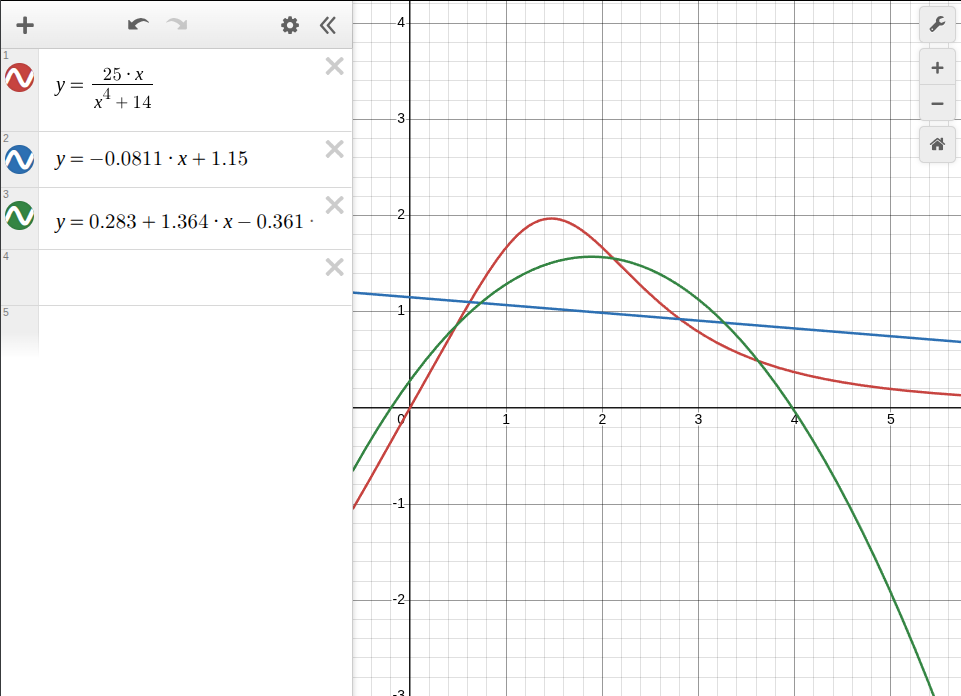
\includegraphics[scale=0.6]{approx_and_function.png}\\
\raggedright
\vspace{5mm}
\section{Программная реализация задачи}
\vspace{5mm}
\url{https://github.com/Ran4er/mystudy/tree/main/4%20computMath/lab_4}\\
\vspace{5mm}
Результаты выполнения программы для различных исходных данных:\\
\begin{lstlisting}[language=Python]
import numpy
\end{lstlisting}
\vspace{5mm}
\section*{Вывод}
В рамках лабораторной работы проведено приближение заданной функции с помощью различных методов аппроксимации: линейной, квадратичной, кубической, экспоненциальной и логарифмической. Для реализации расчётов разработан скрипт на Python, применяющий метод наименьших квадратов и визуализирующий исходные данные вместе с аппроксимирующими кривыми.

В результате анализа определено наилучшее приближение на основе сравнения среднеквадратических отклонений. Дополнительно для линейной зависимости вычислен коэффициент корреляции Пирсона, что позволило оценить тесноту связи между переменными.

\end{document}
